\documentclass[paper-main.tex]{subfiles}


\begin{document}


Continuous gravitational wave signals may wander slowly in frequency over time, due to stochastic internal processes in the superfluid interior of isolated neutron stars~\cite{MelatosDouglassSimula:2015,Jones:2010} or stochastic accretion flows in binary neutron stars~\cite{BildstenTB:1998}. 
The audio analogue of this is a tone that wanders in frequency; a note that changes pitch. 


The analysis techniques used here are inspired by those used to search for continuous waves from spinning neutron in LIGO and Virgo data~\cite{SuvorovaEtAl:2016,SuvorovaEtAl:2017}.
Continuous wave searches are performed on long datasets (months to years in duration). 
The frequency of gravitational-wave emission wanders significantly over the observation period. 
In this context, ``significantly'' means ``across multiple frequency bins'', where the typical width of a frequency bin is the reciprocal of the total observing time~\cite{JKS:1998,ScoX1O2Viterbi:2019}



One method to search for a wandering signal is to split the data into several shorter segments which are analysed individually. 
The detection statistics in every segment are combined to form a grid in time and frequency (spectrogram). 
The value at each spectrogram point determines the likelihood that a signal is present at a particular time and frequency. 
In gravitational-wave data analysis, a detection statistic is used to calculate the likelihood of a signal given the antenna beam pattern of the detector, which varies as the Earth rotates and orbits the Sun~\cite{JKS:1998}.
The detection statistic used depends on the type of target~\cite{JKS:1998,SuvorovaEtAl:2017}. 
In this work the detection statistic is the amplitude (modulus) of the Fourier transform of the data at each time segment, which maximizes the likelihood of detecting a sinusoid in Gaussian noise, as described in Appendix~\ref{app:sinusoid_likelihood}. 
The resulting spectrogram gives the Fourier amplitude for each frequency and time bin. 


In continuous wave searches a hidden Markov model is used to describe the system. 
The frequency (the state) of the signal is unknown (hidden) and the signal is Markovian in that the state at any time depends only on the state in had at the previous time step. 
The hidden Markov model method relates the observable quantity (the detection statistic) to the signal frequency (the hidden state). 
The task is to find the most likely wandering frequency signal given the observable of the spectrogram. 
The Viterbi algorithm~\cite{Viterbi:1967} is an efficient method to find the most likely path of a signal given an observation sequence. 
This method is used in continuous wave searches for a range of astrophysical targets~\cite{ScoX1O2Viterbi:2019,ScoX1ViterbiO1:2017,MillhouseStrangMelatos:2020,JonesSun:2020,MiddletonEtAlO2LMXBs:2020,PostMergerRemnantSearch:2019,SunEtAlSNR:2018,viterbi_application}. 
 



In Section~\ref{sec:viterbi} we review the Viterbi algorithm and its application to this work. 
In Section~\ref{sec:wanderingResults} we present the results for recovery of a wandering audio frequency. 




\subsection{The hidden Markov model and Viterbi algorithm}
\label{sec:viterbi}



The spectrogram grid is indexed by time $t$ and frequency $f$ where there are $N_t$ and $N_f$ time and frequency bins respectively, as shown in Fig.~\ref{fig:viterbi}.
We label the elements of the grid as $t_i$ and $f_j$ with $i=0,1,2,...N_t$ and $j=0,1,2,...,N_f$. 
The normalised Fourier amplitude $F(t_i,f_j)$ is the detection statistic indicating the likelihood that a signal is present in each grid element. 


The objective is to find the most likely path through the grid given the data and any probabilistic constraints on how the frequency wanders from $t_i$ to $t_{i+1}$. 
In continuous wave searches, a physical model is used to decide how much the frequency of the signal is allowed to wander at each time step, which depends on the type of target. 
In this work, at each time step we allow the frequency to either a) stay in the same bin; b) move up a single frequency bin; or c) move down a single frequency bin. 
In a hidden Markov model, the probability of transitioning from $f_j$ at $t_i$ to any of $\{f_{j+1},f_j,f_{j-1}\}$ at $t_{i+1}$ is called the transition probability $A(f_k,f_m)$. 
In this work the three options have equal probability $A(f_k,f_m)=1/3$ for $k=m+1,m,m-1$ and $A(f_k,f_m)=0$ otherwise.


A path through the grid has a likelihood dependent on the detection statistic (the observation) and the transition probability.
If the starting probabilities are all equal, i.e. ${\rm Pr}[f(t_0)] = 1/N_f$, the the probability of the frequency equalling $f(t_{i+1})$ at $t = t_{i+1}$ is defined recursively by
\begin{eqnarray}
{\rm Pr}[f(t_{i+1})=f_j] =~& F[t_{i+1},f(t_{i+1})] \nonumber \\
                     &\times A[f(t_{i+1}),f(t_i)]  \nonumber \\
                     &\times {\rm Pr}[f(t_i)].
\label{eqn:recursiveViterbi}
\end{eqnarray}
The sequence $f(t_0),f(t_1),\dots,f(t_{N_t})$ that maximizes ${\rm Pr}[f(t_{N_t}) = f_j]$ is the optimal Viterbi path terminating in the frequency bin $f_j$. 
We can the maximize the latter quantity over $0 \leq j \leq N_f$ to find the optimal Viterbi path overall, i.e. terminating in any frequency bin. 


The Viterbi algorithm is an efficient method to find the Viterbi path. 
Here we describe the algorithm as pseudo-code referring to the schematic in Fig.~\ref{fig:viterbi}, where the circles indicate the elements of the spectrogram grid (lighter colours correspond to higher likelihood). 
The implementation used in this work is available online (see Appendix~\ref{app:code}).
\begin{enumerate}
\item Starting at $t_1$, each $f_j$ element has three possible paths it could originate from at $t_0$, indicated by the lines in Fig.~\ref{fig:viterbi}. 
At each $f_j$ element, the highest $F[t_0,f_j] A[f(t_0),f(t_1)]$ from the previous time step is selected, highlighted by the black lines in Fig.~\ref{fig:viterbi}. 
For example for the element labelled (a), the highest value is directly behind it, therefore the transition from $\{t_0,f_0\}$ to $\{t_1,f_0\}$ is selected. 
Each element has now selected the best path from the previous time step. 
In Fig.~\ref{fig:viterbi}, black lines show the best paths and grey lines show all other paths. 

\item Moving to $t_2$, the path with the highest value of the recursive relation in Eqn.~\ref{eqn:recursiveViterbi} is selected for each $f_j$ as shown by the solid lines from $t_1$ to $t_2$ in Fig.~\ref{fig:viterbi}. 
The origins are stored for each grid point.

\item Steps 2 is repeated until the end of the grid ($t=t_{N_t}$) is reached. 
Only the best paths are stored. 

\item At $t=t_{N_t}$, each $f_j$ has a value ${\rm Pr}[f(t_{N_t})=f_j]$ (Eqn.~\ref{eqn:recursiveViterbi}). 
The algorithm selects the terminating frequency $f(t_{N_t})$ with the highest value, marked (b) in Fig.~\ref{fig:viterbi}.

\item The Viterbi path is then found by backtracking along the stored best paths at each time step (see also Appendix~\ref{app:viterbi}). 
% come back to this. 
%\jam{[Andrew mentioned providing a closed form here, which I'm not sure exists. The code works by storing three arrays: the weights, the score for the best path to a given vertex, and the index of the previous vertex along that path. Backtracking comprises of looping through that third array from the vertex in the last row with the highest score from the second array. I don't think we need to explain it any further than that.]}
In Fig.~\ref{fig:viterbi}, we see that the path ending at (b) started at (c). 
The Viterbi path is highlighted in orange in Fig.~\ref{fig:viterbi}.
\end{enumerate}
The Viterbi algorithm is an example of a dynamical programming algorithm, where a computation can be broken down into a series of sub-computations.
The Viterbi path for a time series sequences spanning $t_0$ to $t_{N_t}$ contains the Viterbi path for sub-sequences of that time series. 
The algorithm is computationally efficient, at every time step all but $N_f$ possible paths are eliminated (see also Ref.~\cite{ScoX1ViterbiO1:2017}).

\begin{figure}
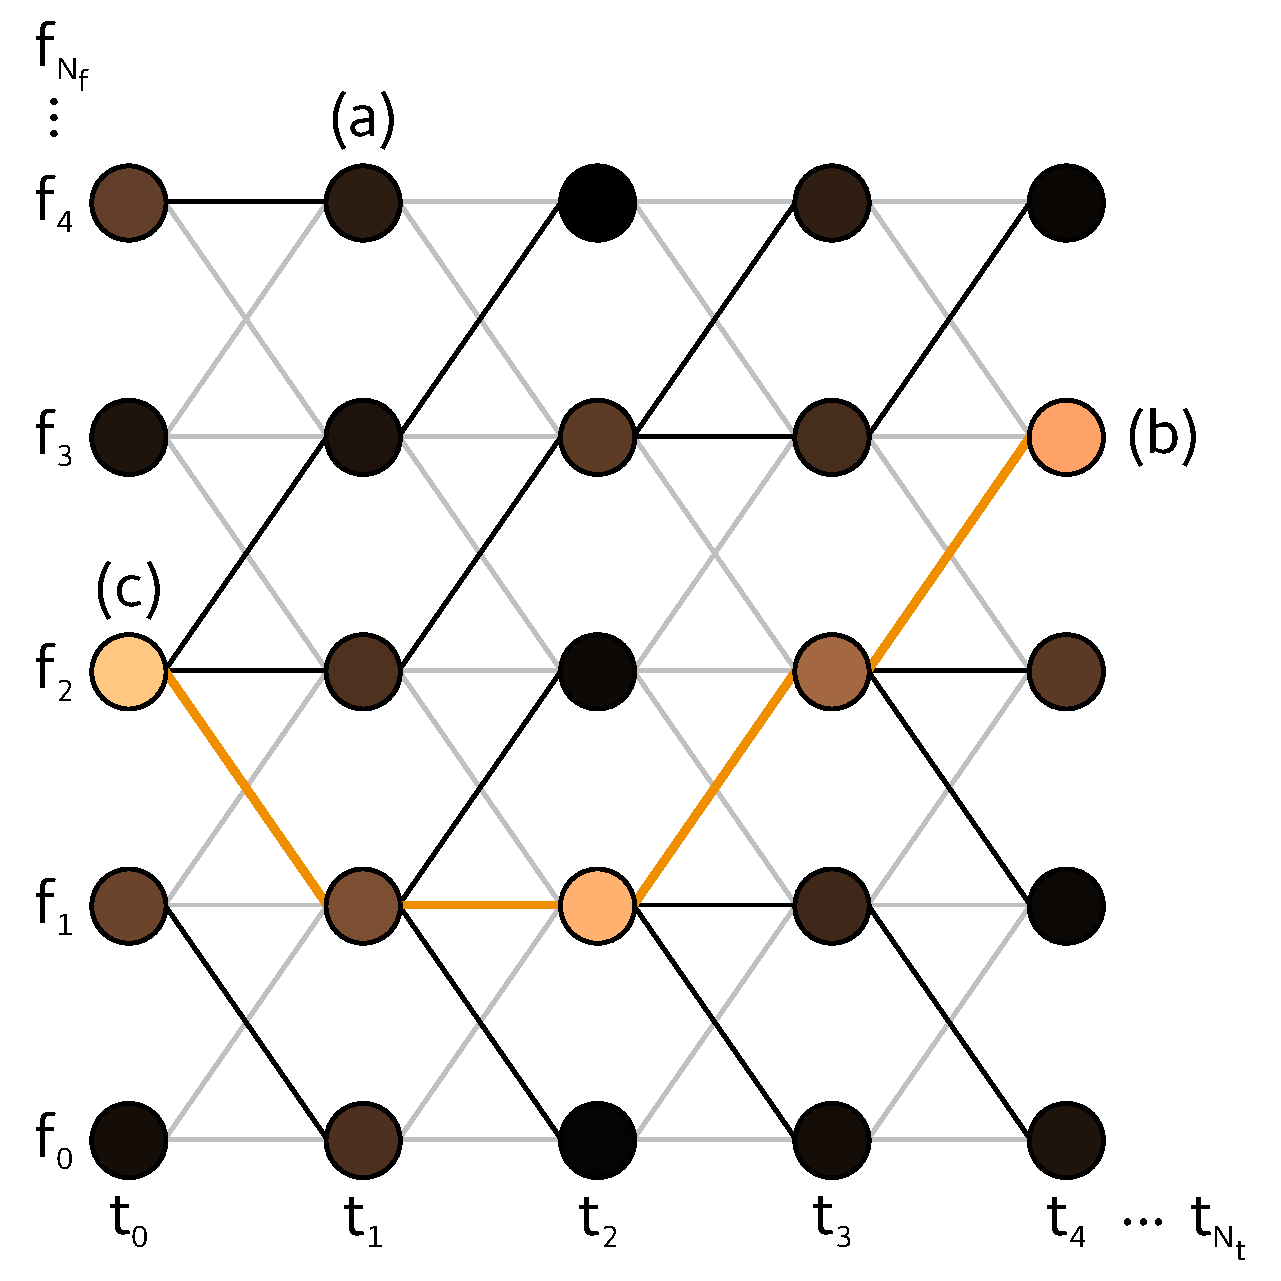
\includegraphics[width=0.49\textwidth]{figures/viterbiDiagram.pdf}
\caption{\label{fig:viterbi}
A schematic diagram of the Viterbi algorithm. 
Each box represents an element in the time-frequency grid starting from the instant $t_0$ on the left and ending at $t_{N_t}$ on the right. 
Vertically, the grid starts from frequency $f_0$ at the bottom and ending at $f_{N_f}$ at the top. 
The colour of each circle indicates the likelihood that a signal is present in the box, where a lighter colour corresponds to higher likelihood. 
AT each time step, the paths can move up one $f$ step, move down one $f$ step, or stay at the same $f$ step (shown by lines in the diagram). 
Each circles has three paths leading to it indicated by the lines. 
The best path to each circle at each $t_i$ is highlighted in black. 
Some routes through the grid are found to be dead ends, such as the path ending at $t_1$ marked (a). 
At $t=t_{N_t}$ the algorithm chooses the terminating frequency circle which has the highest value given by Eqn.~\ref{eqn:recursiveViterbi}, marked (b). 
The Viterbi path is the path leading to this circle, highlighted in orange from (b) to the start at (c). 
}
\end{figure}



\subsection{Sample output}
\label{sec:wanderingResults}

\begin{figure*}
	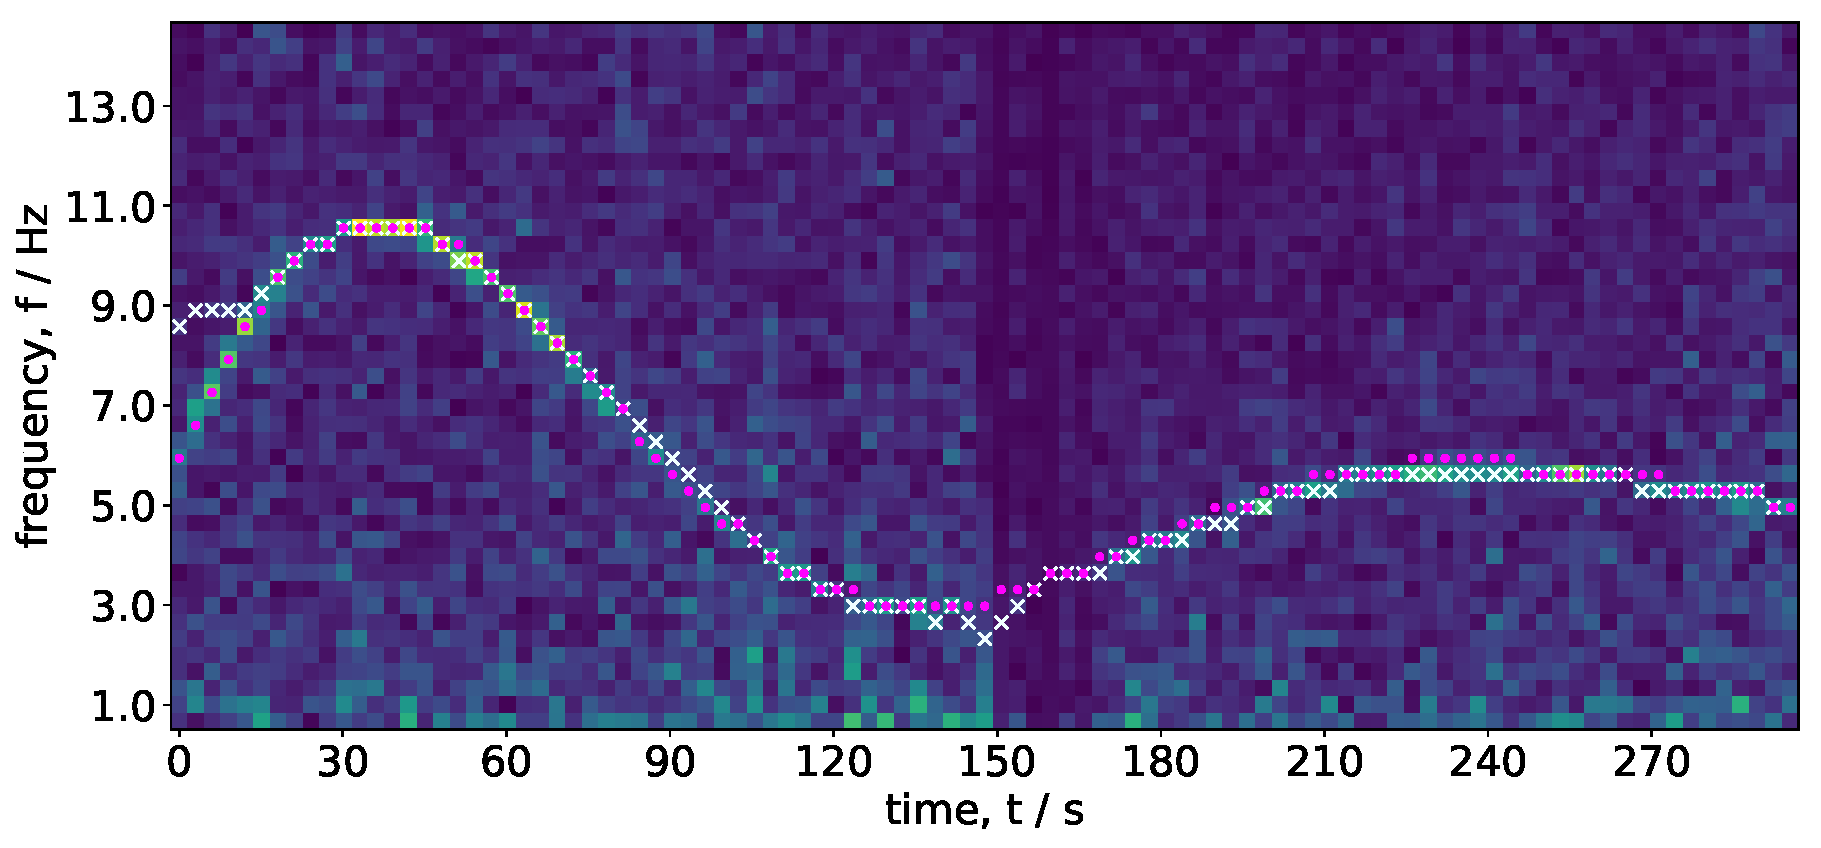
\includegraphics[width=\textwidth]{figures/expt_overlay_2_viterbi_test_webcam.pdf}
	\caption{\label{fig:viterbi_overlay}
Recovery of a wandering tone. 
The spectrogram shows the observed frequency amplitude at each time-frequency step. 
The overlaid pink-dot and white-cross markers show the injected signal and recovered Viterbi path respectively. 
On the left, before $\sim 15\,{\rm s}$, the signal changes frequency too quickly for the Viterbi algorithm to recover. 
At $150\,{\rm s}$ the data appears anomalous, which may be due to some background noise. }
\end{figure*}
 
To test the Viterbi algorithm, a sinusoidal signal with wandering frequency was played through the speaker and the output recorded via webcam as in Section~\ref{sec:single_tone}. 
The injected frequency itself followed a sinusoid with decaying amplitude. 
This choice was arbitrary, any injected path would have worked, as long as it changed slowly enough for the search parameters of the algorithm.



The results are shown in Fig.~\ref{fig:viterbi_overlay}, where the heatmap shows the spectrogram of the observed signal. 
The overlaid pink-dot markers show the injected signal. 
The white-cross markers show the recovered Viterbi path maximised over all terminating frequency bins, which qualitatively provides a good match to the injection. 
Initially, the injected signal moves faster than the frequency wander limit, leading to the discrepancy observed for $t\lesssim 10\,{\rm s}$. 
There is also an anomaly at $150\,{\rm s}$, which illustrates what happens when the interferometer is disturbed, e.g. when someone walks nearby. 
The Viterbi algorithm is robust against such disturbances, recovering the optimal path promptly, as Fig.~\ref{fig:viterbi_overlay} shows. 


Quantitatively, the Viterbi path is within one frequency bin ($\approx 0.3\,{\rm Hz}$) of the injected signal for $94\%$ of the time. 
Another figure of merit is the root mean square (RMS) fractional error $E_{\rm rms}$ along the path defined as 
\han{}
\begin{equation}
E_{\rm rms} = \left[ \frac{1}{N_t+1} \sum_{i=0}^{N_t} \frac{(I_i - R_i)^2}{{I_i}^2} \right] ^{1/2}
\end{equation}
where $I_i$ and $R_i$ are the injected and recovered (Viterbi) frequency paths. 
Computing this for the result shown in Fig.~\ref{fig:viterbi_overlay} we find $E_{\rm rms} = 0.082$, which indicates fair but not total recovery of the injected signal.


\end{document}
